\documentclass[a4paper]{scrreprt}
\setcounter{tocdepth}{3}
\setcounter{secnumdepth}{3}

\usepackage[german]{babel}
\usepackage[utf8]{inputenc}
\usepackage[T1]{fontenc}
\usepackage{ae}
\usepackage{graphicx}
\usepackage{tabu}

\begin{document}
\title{Entwurf}
\author{Fangzhou Bian, Kathrin Blum, Matthias Bruns, \\Leonhard Duda, Tan Grumser, Yuguang Lin}
\maketitle
%\Footnote für Fußnoten
% Platzierung des Inhaltsverzeichnisses
\tableofcontents



\chapter{Einleitung}

\chapter{Grobentwurf}
\section{Systemarchitektur}
Die App MensaMeet wird als Client-Server Anwendung umgesetzt. Clients fordern Dienste an, welche vom zentralen Server bereitgestellt werden. Dazu hat jeder Client, nachdem er sich einmal registriert hat, eine eindeutige User-ID. Der Server verwaltet eine Datenbank, in welcher User- und Gruppeninformationen gehalten werden. 
Die Client-Seite der Anwendung wird mithilfe der MVVM (Model-View-Viewmodel) Architekur umgesetzt.
Die Server-Seite mithilfe der MVC (Model-View-Control) Architektur.

\subsection{Client}
Die Client Seite bedient sich der MVVM Architektur. Die View dient zum anzeigen von Daten, sie beinhaltet alle grafischen Elemente, stellt also die GUI dar. Im Model werden die Daten gehalten und Funktionen zur Manipulation der Daten bereitgestellt.
Das Viewmodel enthält die Darstellungslogik für die View und kapselt sie von der Anwendungslogik, die sich im Model befindet, ab.
View und Viewmodel sind durch Databinding nur lose gekoppelt. Dadurch kann die View problemlos ausgetauscht werden bzw. können mehrere verscheidene Views (z.b. angepasst an Tablet, Desktop,...) zum selben Viewmodel existieren.
Das Datainding kann als bidirektionaler Beobachter verstanden werden. Die lose Kopplung verbessert die Testbarkeit.

\subsection{Server}
Für die Server Seite wird die MVC Architektur verwendet.
Das Model ist für die Datenhaltung zuständig und beinhaltet/verwaltet eine Datenbank.  (In unserem Fall wird MySQL verwendet, als Kommunikationsschnittstelle zwischen der Datenbank und den Controllern wollen wir JPA mit Hibernate benutzen).
View ist durch eine Schnittstelle gegeben, über die der Server Anfragen des Client empfängt und an den Controller delegiert. Der Controller führt diese Anfragen durch, indem er angefordere Daten aus dem Model holt oder neue Daten einfügt bzw Daten anpasst.
\section{Systemkomponenten}
\section{Komponentenbeschreibung}
\subsection{Client}
\subsection{Server}


\chapter{Feinentwurf}
\section{Klassen des Clients}
\subsection{Klassendiagramm}

\subsubsection{Muster}

\section{Klassen des Server}
\subsection{Klassendiagramm}
\subsection{package.edu.kit.mensameet.models}
\subsubsection{Class User}
\subsubsection*{Beschreibung}
Diese Klasse beschreibt einen User 

\subsubsection*{Konstruktor}
public User(String name, String password)

\subsubsection*{Methoden}
\begin{addmargin}[25pt]{0pt}

\subsubsection*{Paramter}
\begin{itemize}
\item
\item
\item
\end{itemize}

\subsubsection*{Rückgabewert}
\end{addmargin}


%------------ Java Doc for the sever view package ---------------------


\subsection{package.edu.kit.mensameet.view}

Alle folgenden Klassen haben keine Konstruktoren, da sie keine Instanzen besitzen sollen,sondern lediglich statische Funktionen beinhalten, die die Schnittstelle des Servers bilden.

\subsubsection{Class UserService}
\subsubsection*{Beschreibung}
Diese Klasse stellt die für den Client benötigten Funktionen bereit um User Daten abzufragen und zu bearbeiten. 

\subsubsection*{Methoden}
\begin{addmargin}[25pt]{0pt}

\subsubsection*{Paramter}
\begin{itemize}
\item
\item
\item
\end{itemize}

\subsubsection*{Rückgabewert}
\end{addmargin}

%---------------------

\subsubsection{Class UserService}
\subsubsection*{Beschreibung}
Diese Klasse stellt die für den Client benötigten Funktionen bereit um User Daten abzufragen und zu bearbeiten. 

\subsubsection*{Konstruktor}
public User(String name, String password)

\subsubsection*{Methoden}
\begin{addmargin}[25pt]{0pt}

\subsubsection*{Paramter}
\begin{itemize}
\item
\item
\item
\end{itemize}

\subsubsection*{Rückgabewert}
\end{addmargin}



%-------------- Java Doc for the server controller package --------------



\subsection{package.edu.kit.mensameet.services}
\subsubsection{Class UserServices}
\subsubsection*{Beschreibung}
Die Klasse beinhaltet die für den User zuständigen Services

\subsubsection*{Methoden}
\begin{addmargin}[25pt]{0pt}
\begin{itemize}

\item Public User getUserById(String userId)\\
	Anfrage auf ein User Profil mit der gegebenen und eindeutigen User ID
	\subsubsection*{Parameter}
	\begin{itemize}
	\item userId \\
		Eindeutige ID eines Userprofils
	\end{itemize}
	\subsubsection*{Rückgabewert}
	\begin{itemize}
	\item User Profil mit allen Parametern 
	\end{itemize}

\item Public User addUser(User user)\\
	Hinzufügen eines Users zur Datenbank
	\subsubsection*{Parameter}
	\begin{itemize}
	\item user \\
		Eindeutiges User Profil
	\end{itemize}
	\subsubsection*{Rückgabewert}
	\begin{itemize}
	\item User Profil
	\end{itemize}
	
\item Public bool removeUser(String userId)\\
	User Profil aus der Datenbank löschen
	\subsubsection*{Parameter}
	\begin{itemize}
	\item userId \\
		Eindeutige ID eines User Profils
	\end{itemize}
	\subsubsection*{Rückgabewert}
	\begin{itemize}
	\item True falls User Profil erfolgreich gelöscht wurde und false falls nicht
	\end{itemize}
\end{itemize}
\end{addmargin}

\subsubsection{Class GroupService}
\subsubsection*{Beschreibung}
Diese Klasse beschreibt alle für Gruppen zuständige Services

\subsubsection*{Methoden}
\begin{addmargin}[25pt]{0pt}
\begin{itemize}

\item Public Group getGroupById(String groupId)\\
	Anfrage nach einer Gruppe mit der gegebenen und eindeutigen Gruppen ID
	\subsubsection*{Parameter}
	\begin{itemize}
	\item groupId \\
		Eindeutige Gruppen ID
	\end{itemize}
	\subsubsection*{Rückgabewert}
	\begin{itemize}
	\item Gruppe 
	\end{itemize}
	
\item Public Group addGroup(Group group)\\
	Hinzufügen einer Gruppe zur Datenbank
	\subsubsection*{Parameter}
	\begin{itemize}
	\item group \\
		Gruppe mit korrekten Parametern
	\end{itemize}
	\subsubsection*{Rückgabewert}
	\begin{itemize}
	\item Hinzugefügte Gruppe 
	\end{itemize}
	
\item Public Group[] getGroupByPreferences(Preferences prefs)\\
	Abfrage nach Gruppen mit passenden Präferenzen
	\subsubsection*{Parameter}
	\begin{itemize}
	\item prefs \\
		Nötige Präferenzen zur Findung einer passenden Gruppe(Linie und Uhrzeit)
	\end{itemize}
	\subsubsection*{Rückgabewert}
	\begin{itemize}
	\item Alle Gruppen mit übereinstimmenden Präferenzen
	\end{itemize}

\item Public bool removeGroup(String groupId)\\
	Löscht Gruppe aus der Datenbank
	\subsubsection*{Parameter}
	\begin{itemize}
	\item groupId \\
		Eindeutige Gruppen ID der zu löschenden Gruppe
	\end{itemize}
	\subsubsection*{Rückgabewert}
	\begin{itemize}
	\item true falls die Gruppe erfolgreich gelöscht wurde und false wenn nicht
	\end{itemize}
\end{itemize}
\end{addmargin}

\subsubsection{Class MensaLineDataService}
\subsubsection*{Beschreibung}
Diese Klasse enthält die Services die für die Verwaltung der Mensadaten zuständig sind

\subsubsection*{Methoden}
\begin{addmargin}[25pt]{0pt}
\begin{itemize}

\item Public LineData[] grablineData()\\
	Abfrage des tagesaktuellen Speiseplans aller Linien vom Studentenwerk

	\subsubsection*{Rückgabewert}
	\begin{itemize}
	\item Array aller Linien 
	\end{itemize}
	
\item Public LineData[] getLineData()\\
	Abrufen der des tagesaktuellen Speiseplans aller Linien aus der Datenbank
	\subsubsection*{Rückgabewert}
	\begin{itemize}
	\item Array aller Linien
	\end{itemize}
\end{itemize}
\end{addmargin}

\subsubsection{Class MembershipService}
\subsubsection*{Beschreibung}
Diese Klasse beinhaltet die Services die sich um die Gruppenmitgliedschaft der einzelnen User kümmert

\subsubsection*{Methoden}
\begin{addmargin}[25pt]{0pt}
\begin{itemize}

\item Public bool addUserToGroup(String UserId, String groupId)\\
	Fügt einen User zu einer Gruppe hinzu
	\subsubsection*{Parameter}
	\begin{itemize}
	\item userId \\
		Eindeutige ID des Users der hinzugefügt werden soll
	\item groupId \\
		Eindeutige ID der Gruppe zu der der User hinzugefügt werden soll
	\end{itemize}
	\subsubsection*{Rückgabewert}
	\begin{itemize}
	\item true falls erfolgreich hinzugefügt und false falls nicht
	\end{itemize}
	
\item Public bool removeUserFromGroup(String userId, String groupId)\\
	Beendet die Zugehörigkeit eines Mitglieds zu einer Gruppe
	\subsubsection*{Parameter}
	\begin{itemize}
	\item userId \\
		Eindeutige ID des Users der aus der Gruppe entfernt werden soll
	\item groupId \\
		Eindeutige ID der Gruppe aus der der User entfernt werden soll
	\end{itemize}
	\subsubsection*{Rückgabewert}
	\begin{itemize}
	\item true falls erfolgreich aus der Gruppe entfernt und false falls nicht
	\end{itemize}
\end{itemize}
\end{addmargin}

\subsubsection{Class UserProfilService}
\subsubsection*{Beschreibung}
Diese Klasse beinhaltet den Service zum Bearbeiten eines User Profils

\subsubsection*{Methoden}
\begin{addmargin}[25pt]{0pt}
\begin{itemize}

\item Public bool updateUserProfile(User user)\\
	Überschreibt bereits vorhandenes User Profil mit neuem Profil (ID bleibt unverändert)
	\subsubsection*{Parameter}
	\begin{itemize}
	\item user \\
		User Profil mit veränderten Parametern
	\end{itemize}
	\subsubsection*{Rückgabewert}
	\begin{itemize}
	\item true falls erfolgreich geändert und false falls nicht
	\end{itemize}

\end{itemize}
\end{addmargin}


\section{HTTP Protokoll}

Die REST Endpoints die in der Tabelle aufgelistet sind werden für die Kommunikation zwischen Client und Server verwendet. \\

\resizebox{16cm}{!} {
\begin{tabu} { | l | l | l | l | } 
 \hline
 Request Type & Endpoint & Payload & Beschreibung \\ [0.5ex] 
 \hline
 GET  & /user/\{token\} &  & Liefert den User mit dem übergebenem Token. \\ 
 
 POST & /user  & User & Updated den User (Token liegt in User) \\ 
 \hline
GET & /group/{token} & & Liefert die Gruppe mit dem übergebenem Token. \\
POST & /group-prefferences & Preferrences & Liefert alle Gruppen die zu den übergebenen Prefferenzen passen. \\
POST  & /create-group/  & Group & Erstellt die übergebene Gruppe. \\
DELETE  & /group/\{token\} & & Löscht die Gruppe mit dem übergebenen Token. \\

\hline 

POST  & /add-user-to-group?user=\{userToken\}\&group={groupToken} & & Fügt den User mit dem userToken zu der Gruppe mit dem groupToken. \\
POST  & /remove-user-from-group?user=\{userToken\}\&group={groupToken} & & Entfernt den User mit dem userToken von der Gruppe mit dem groupToken. \\

\hline

POST & /login & email, password & Meldet den Client an dem Account mit den übergebenen Anmeldedaten an. \\
POST & /register & email, password & Erstellt einen Account mit den übergebenen Anmeldedaten. \\

\hline

GET &  /mensadata & & Liefert die aktuellen Mensadaten.\\

\hline

\end{tabu}
}




\chapter{Datenstrukturen}

\chapter{Dynamische Modelle}
\section{Aktivitätsdiagramm}

\section{Sequenzdiagramm}
\subsection{Registrieren}
\begin{center}
	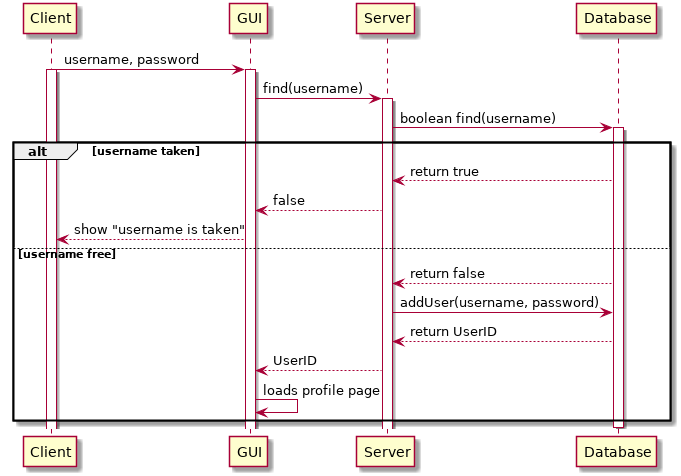
\includegraphics[width=0.93\textwidth]{Sequenzdiagramme/Registration.png}
\end{center}
\subsection*{Beschreibung}
Bob öffnet zum ersten mal die Applikation MensaMeet und sieht den Registrierungsbildschrim. Dort soll er seine E-Mailadresse und ein Passwort eingeben. Sobald er das getan hat, werden die Daten an der Server geschickt, welcher sie an Firebase weiterleitet. Firebase legt auf seinem Server den User an und generiert ein Token zur UserIdentifikation. Das Token wird an den Server zurückgegeben, der damit einen User in der Datenbank anlegt und das Userobjekt an den Client schickt. Auf dem Client (Bobs Smartphone) wird der User/Token gespeichert und bei jeder zukünftigen Anfrage an den Server mitgegeben. 
Bob sieht nun den Bildschirm zur Profilbearbeitung. Die Eingabe der Profildaten ist Pflicht, vorher kann er nicht weiter zu einer anderen Seite gelangen.
Nachdem er seinen Nutzernamen, Motto, Alter, Geschlecht, Status, Fachrichtung eingegeben hat, werden diese Daten an den Server gesendet, der damit das Userprofil in der Datenbank aktualisiert. 
\newpage
\subsection{Mensalinien wählen}
\begin{center}
	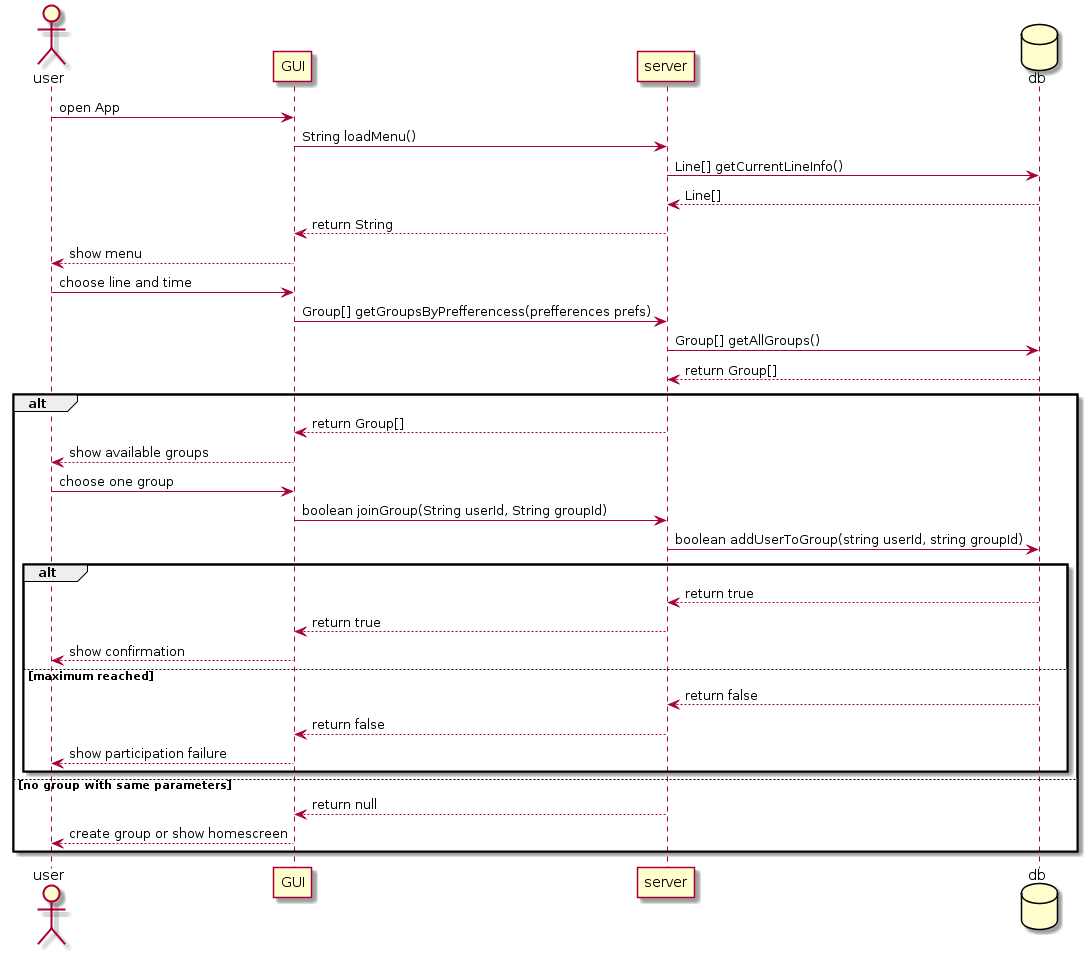
\includegraphics[width=0.93\textwidth]{Sequenzdiagramme/chooseLineAndTimeSD.png}
\end{center}
\subsection*{Beschreibung}
Der Nutzer öffnet die Anwendung (die Registrierung ist bereits erfolgt). Nun soll er als Scrolldown-menü die Mensalinien mit ihrem jeweiligen Angebot zu sehen kriegen (Dies ist der "HomeScreen"). Dazu werden die Mensadaten über den Server von der Datenbank angefragt, aufbereitet und dem Client übermittelt. Dieser kann nun die Linien anklicken an denen er gern essen möchte. Danach stellt er das für ihn geeignete Zeitintervall ein. Diese Daten werden dem Server übermittelt, welcher sich die Gruppen aus der Datenbank holt, nach den angegebenen Daten filtert und an den Client übergibt. Der Nutzer kann sich die Gruppen anschauen und einer davon beitreten. Beim Versuch beizutreten wird dem Server der User- und der GroupToken übermittelt. Es wird überprüft ob die Gruppe bereits voll ist, ist dies der Fall, erhält der Client eine Fehlermeldung und gelangt wieder zur Gruppenübersicht. Ist noch Platz in der Gruppe, wird die Gruppe in der Datenbank aktualisiert, indem der User hinzugefügt wird. Dann wird über den Server eine Bestätigung an den Client geschickt und der Nutzer gelangt zur Gruppenseite. 
Falls keine Gruppen passend zu den Angaben des Clients gefunden wurde, erhält der Client eine passende Fehlermeldung und kann entweder zurück zum HomeScreen oder selbst eine Gruppe erstellen.

\newpage
\subsection{Gruppe beitreten}
\begin{center}
	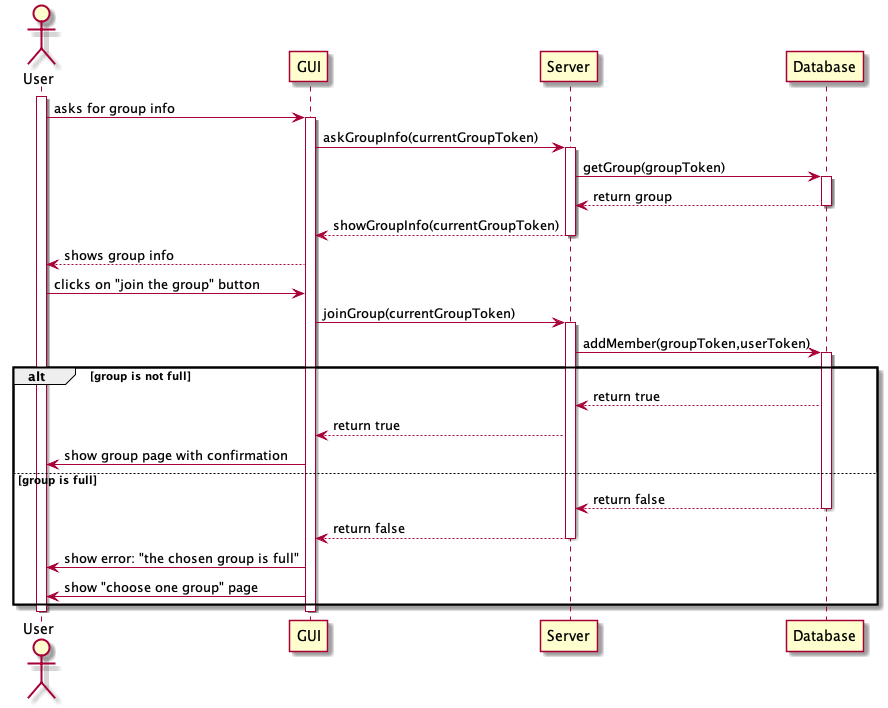
\includegraphics[width=0.93\textwidth]{Sequenzdiagramme/checkInfoAndJoinGroupSD.png}
\end{center}


\subsection*{Beschreibung}
Nachdem der Nutzer, passend zu seinen ausgewählten Linien und seinem eingestellten Zeitintervall, Gruppen in einem Scrolldown-menü angezeigt bekam, klickt er nun eine Gruppe an, um mehr Informationen zu ihr zu sehen. Dazu wird an den Server eine Anfrage mit dem GroupToken gesendet. Der Server sucht damit nach der Gruppe in der Datenbank und übermittelt die Informationen dem Client. Beim User wird die angeklickte Gruppe nach unten aufgklappt, so dass nun zusätzlich zur Linie, Startzeit und Motto auch die Mitgliederliste und den "Beitreten"-Button sieht. Er drückt auf "Beitreten". Nun wird dem Server die UserID und GroupID übermittelt. Er prüft in der Datenbank ob die Gruppe inzwischen voll ist. Ist dies der Fall, erhält der Client eine Fehlermeldung : "Deine gewählte Gruppe ist bereits voll" und gelangt wieder zur Gruppenübersicht. Ist noch Platz in der Gruppe, wird die Datenbank aktualisiert und dem Client der Beitritt bestätigt. Der Nutzer gelangt zur Detailansicht seiner Gruppe. Er steht nun ebenfalls in der Mitgliederliste und sieht den Button "Gruppe Verlassen".

\newpage
\subsection{Gruppe erstellen}
\begin{center}
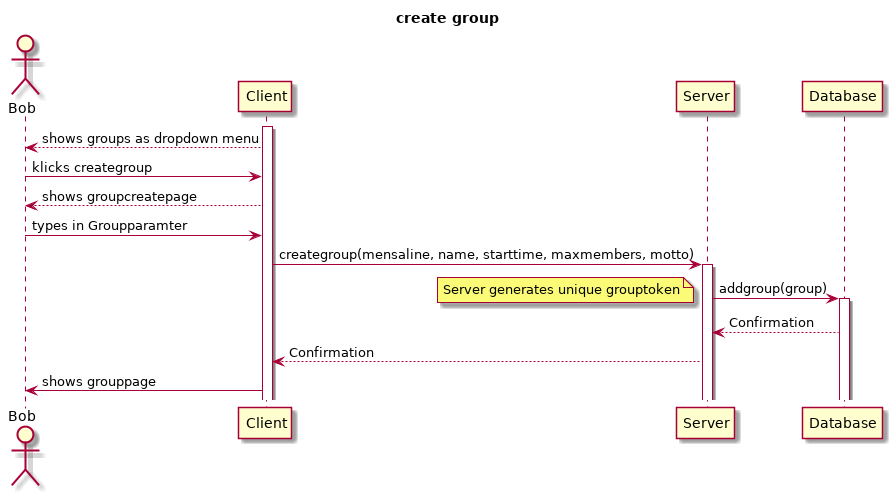
\includegraphics[width=0.93\textwidth]{Sequenzdiagramme/CreateGroup.png}

\end{center}
\subsection*{Beschreibung}
Nachdem der User die zu ihm passenden Gruppen angefragt hat, aber keine gefunden wurde entscheidet er sich eine Gruppe zu erstellen. Er stellt dazu die erforderlichen Gruppenparameter(Gruppenname, Mensalinie, Startzeit, Motto, Maximale Mitgliederzahl) ein. Der Server erhält die Anfrage mit diesen Paramtern eine neue Gruppe anzulegen. Er generiert (aus dem Namen?) ein eindeutiges groupToken und legt die Gruppe in der Datenbank an. Dem Client wird die erfolgreiche Gruppengründung bestätigt und ihm wird als nächstes die Detailansicht seiner Gruppe angezeigt.

\newpage
\subsection{Gruppe verlassen}
\begin{center}
	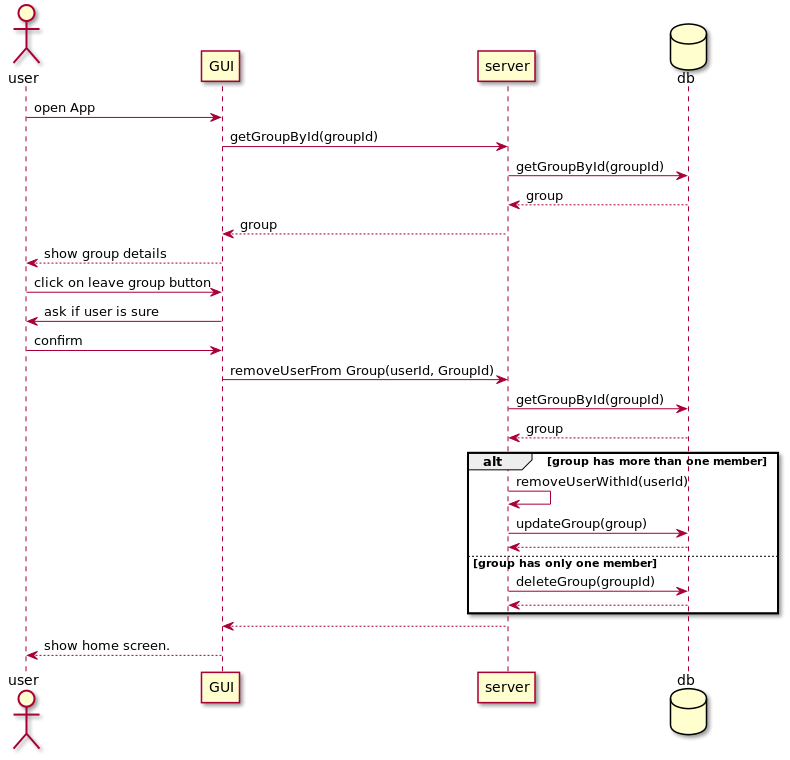
\includegraphics[width=0.93\textwidth]{Sequenzdiagramme/leaveGroupSD.png}
\end{center}

\subsection*{Beschreiung}
Der Nutzer öffnet die App MensaMeet. Da er bereits Mitglied einer Gruppe ist, wird ihm die Detailansicht seiner Gruppe angezeigt.
In dieser Ansicht ist ein Button "Gruppe verlassen". Er drückt diesen Button und muss seine Entscheidung bestätigen. Für den Austritt wird dem Server der User- und GroupToken übermittelt. Der Server sucht anhand des GroupToken die Gruppe in der Datenbank um sie zu aktualisieren. Der User wird aus der Gruppe entfernt und die Mitgliederzahl der Gruppe überprüft. Ist diese nun bei 0, so wird die Gruppe aus der Datenbank gelöscht.
Der Client erhält in jedem Fall die Bestätigung zum Austritt aus der Gruppe und wird wieder zum HomeScreen überführt.


\chapter{Änderungen zum Pflichtenheft}
\begin{itemize}
	\item Nutzername und Gruppennamen müssen nicht mehr eindeutig sein \\
	stattdessen wird für den Nutzer von Firebase ein eindeutiges Token generiert, das als Identifikator dient. Für Gruppen wird ebenfalls ein eindeutiges Token durch den Server generiert.
	\item Zum Registrieren wird statt Nutzername und Password nun Email und Passwort benötigt. \\Diese Änderung ist bedingt durch die Nutzung von Firebase und erfüllt damit eines unserer Wunschkriterien: Dass eine Email Verifikation beim Registrieren stattfindet. 
\end{itemize}

\chapter{Glossar}

\chapter{Anhang}

\end{document}
